Alternativa é simples, $H_1: \theta = \theta_1$, então o melhor teste é chamado de mais poderoso (MP).

\begin{center}
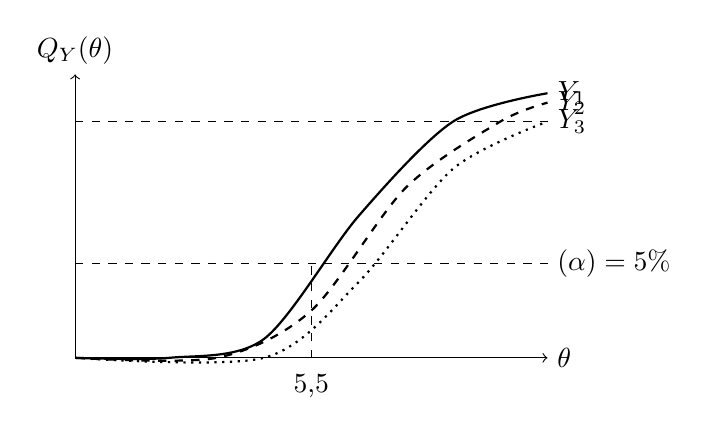
\begin{tikzpicture}[scale=1.2]
    % Eixos
    \draw[->] (0,0) -- (5,0) node[right] {$\theta$};
    \draw[->] (0,0) -- (0,3) node[above] {$Q_Y(\theta)$};
    
    % Linhas horizontais
    \draw[dashed] (0,2.5) -- (5,2.5);
    \draw[dashed] (0,1) -- (5,1) node[right] {$(\alpha) = 5\%$};
    
    % Curvas
    \draw[thick] plot[smooth] coordinates {(0,0) (1,0) (2,0.2) (3,1.5) (4,2.5) (5,2.8)} node[right] {$Y_1$};
    \draw[dashed, thick] plot[smooth] coordinates {(0,0) (1.5,0) (2.5,0.5) (3.5,1.8) (4.5,2.5) (5,2.7)} node[right] {$Y_2$};
    \draw[dotted, thick] plot[smooth] coordinates {(0,0) (2,0) (3,0.8) (4,2) (5,2.5)} node[right] {$Y_3$};
    
    % Linha vertical em 3.5
    \draw[dashed] (2.5,0) -- (2.5,1);
    \node at (2.5,-0.3) {5,5};
\end{tikzpicture}

Comportamento de $Y \in C$ para testar $H_0: \theta = 5,5$
\end{center}

\textbf{Teste simples x simples}

Considere o objetivo de derivar o teste MP para hipóteses do tipo simples x simples via o lema de Neyman e Pearson (1933).

Sejam $\mathbf{X} = (X_1, \ldots, X_n)^T$ uma a.a. de $X$ com fdp (ou fmp) $f(x; \theta)$ para $x \in \mathbb{R}^n$, $\theta \in \Theta \subset \mathbb{R}$ e $\alpha = (x_1, \ldots, x_n)^T$ uma a.o. Desejamos testar

\begin{equation}
H_0: \theta = \theta_0 \quad \times \quad H_1: \theta = \theta_1
\end{equation}

em que $\theta_0, \theta_1 \in \Theta$ e $\theta_0 \neq \theta_1$. Seja $\hat{x}$ a função de verossimilhança associada à hipótese $H_i$.
